\documentclass[11pt,border=6pt]{standalone}
\usepackage{fontspec}
\usepackage{tikz}
\usetikzlibrary{positioning,arrows.meta,calc,fit,backgrounds}
\begin{document}
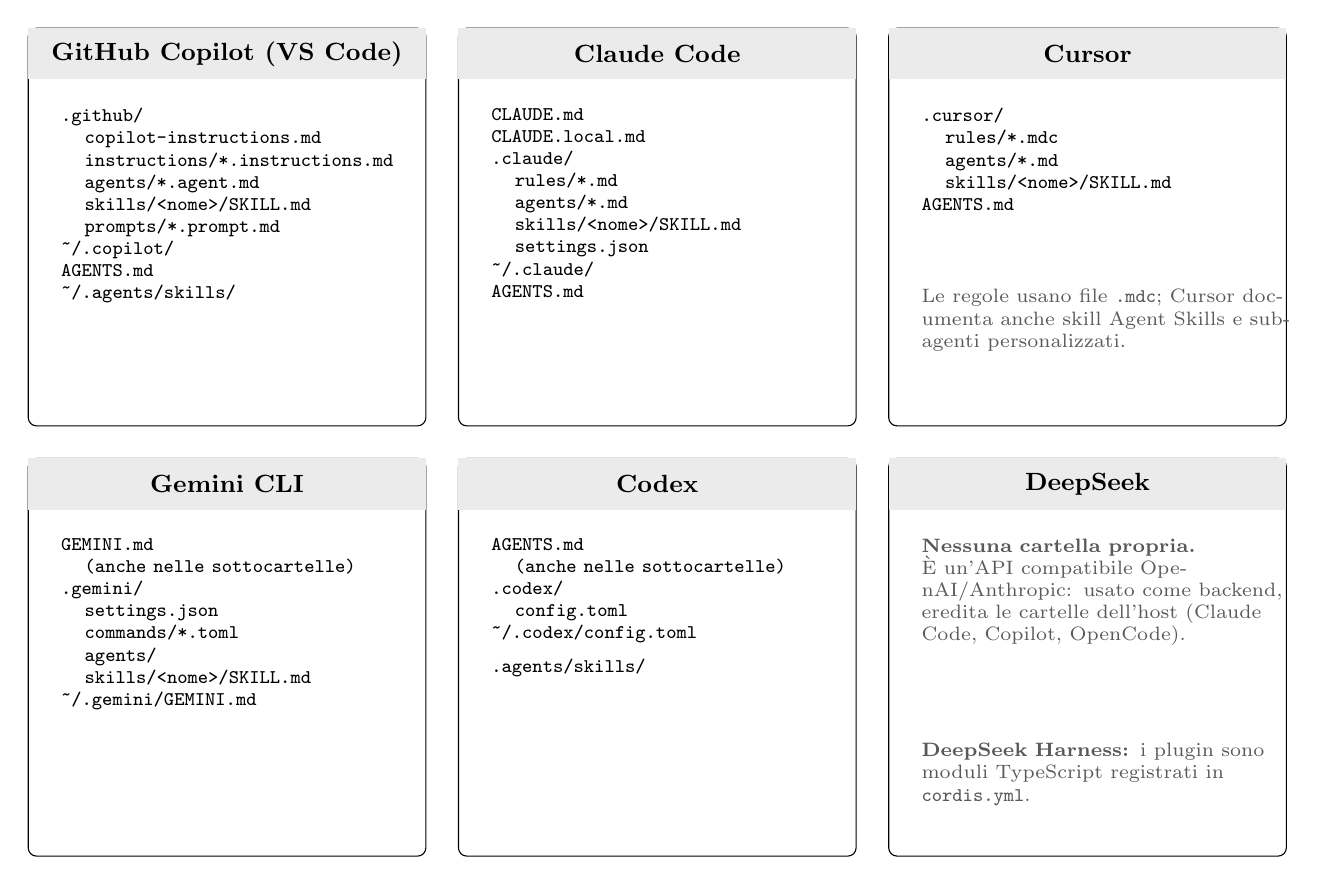
\begin{tikzpicture}[font=\footnotesize,
  card/.style={draw, rounded corners=3pt, minimum width=5.05cm, minimum height=5.05cm, align=left, inner sep=0pt},
  head/.style={fill=black!8, minimum width=5.05cm, minimum height=6.5mm, align=center,
    font=\small\bfseries, inner sep=2pt},
  p/.style={font=\ttfamily\scriptsize, anchor=north west, align=left},
  n/.style={font=\scriptsize, text=black!65, anchor=north west, align=left}]

  % --- riga 1 ---
  \node[card] (c1) at (0,0) {};
  \node[head, anchor=north] at (c1.north) {GitHub Copilot (VS Code)};
  \node[p, text width=4.75cm] at ([xshift=3mm,yshift=-9mm]c1.north west) {.github/\\\hspace*{3mm}copilot-instructions.md\\\hspace*{3mm}instructions/*.instructions.md\\\hspace*{3mm}agents/*.agent.md\\\hspace*{3mm}skills/<nome>/SKILL.md\\\hspace*{3mm}prompts/*.prompt.md\\\textasciitilde/.copilot/\\AGENTS.md\\\textasciitilde/.agents/skills/};

  \node[card, right=4mm of c1] (c2) {};
  \node[head, anchor=north] at (c2.north) {Claude Code};
  \node[p, text width=4.75cm] at ([xshift=3mm,yshift=-9mm]c2.north west) {CLAUDE.md\\CLAUDE.local.md\\.claude/\\\hspace*{3mm}rules/*.md\\\hspace*{3mm}agents/*.md\\\hspace*{3mm}skills/<nome>/SKILL.md\\\hspace*{3mm}settings.json\\\textasciitilde/.claude/\\AGENTS.md};

  \node[card, right=4mm of c2] (c3) {};
  \node[head, anchor=north] at (c3.north) {Cursor};
  \node[p, text width=4.75cm] at ([xshift=3mm,yshift=-9mm]c3.north west) {.cursor/\\\hspace*{3mm}rules/*.mdc\\\hspace*{3mm}agents/*.md\\\hspace*{3mm}skills/<nome>/SKILL.md\\AGENTS.md};
  \node[n, text width=4.75cm] at ([xshift=3mm,yshift=-32mm]c3.north west) {Le regole usano file \texttt{.mdc}; Cursor documenta anche skill Agent Skills e subagenti personalizzati.};

  % --- riga 2 ---
  \node[card, below=4mm of c1] (c4) {};
  \node[head, anchor=north] at (c4.north) {Gemini CLI};
  \node[p, text width=4.75cm] at ([xshift=3mm,yshift=-9mm]c4.north west) {GEMINI.md\\\hspace*{3mm}(anche nelle sottocartelle)\\.gemini/\\\hspace*{3mm}settings.json\\\hspace*{3mm}commands/*.toml\\\hspace*{3mm}agents/\\\hspace*{3mm}skills/<nome>/SKILL.md\\\textasciitilde/.gemini/GEMINI.md};

  \node[card, below=4mm of c2] (c5) {};
  \node[head, anchor=north] at (c5.north) {Codex};
  \node[p, text width=4.75cm] at ([xshift=3mm,yshift=-9mm]c5.north west) {AGENTS.md\\\hspace*{3mm}(anche nelle sottocartelle)\\.codex/\\\hspace*{3mm}config.toml\\\textasciitilde/.codex/config.toml\\[4pt].agents/skills/};

  \node[card, below=4mm of c3] (c6) {};
  \node[head, anchor=north] at (c6.north) {DeepSeek};
  \node[n, text width=4.75cm] at ([xshift=3mm,yshift=-9mm]c6.north west) {\textbf{Nessuna cartella propria.} È un'API compatibile OpenAI/Anthropic: usato come backend, eredita le cartelle dell'host (Claude Code, Copilot, OpenCode).};
  \node[n, text width=4.75cm] at ([xshift=3mm,yshift=-35mm]c6.north west) {\textbf{DeepSeek Harness:} i plugin sono moduli TypeScript registrati in \texttt{cordis.yml}.};
\end{tikzpicture}
\end{document}
